\%!TEX root=../document.tex

\section{Hardware-Aufbau}
\label{sec:Hardware-Aufbau}

asdfg \cite{brands11}

\begin{figure}[!htb]
	\centering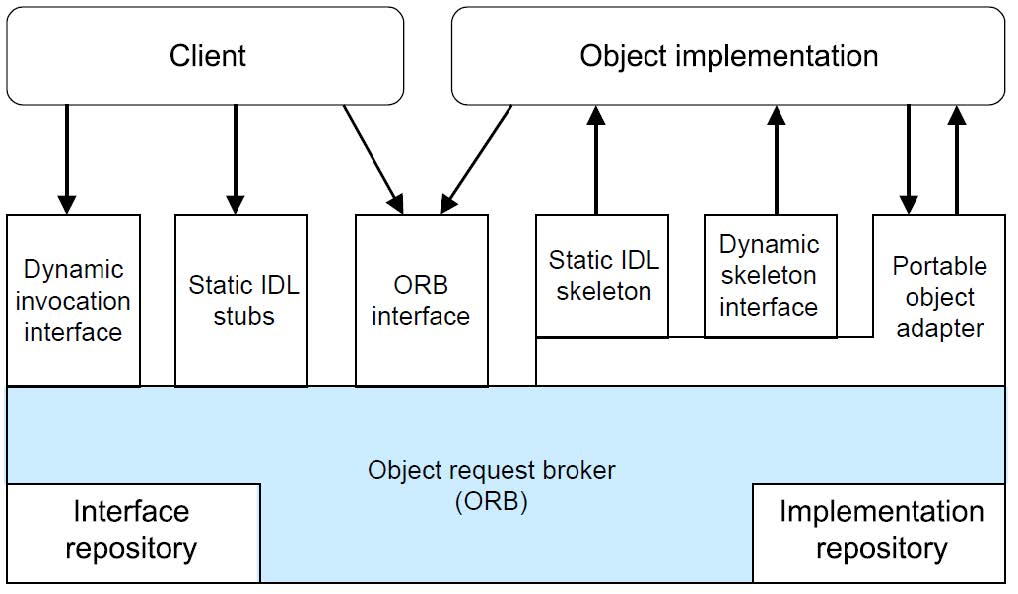
\includegraphics[width=0.8\textwidth]{images/corba.jpg}
	\caption{Ein Corba Bild}
	\label{corba}
\end{figure}

\begin{itemize}
    \item asdf
\end{itemize}


\subsection{Qubit}
\label{sec:Qubit}

## Schroedinger

Schroedingers Katze ist die ber\"uhmteste Veranschaulichung eines grundlegenden Ph\"anomens der Quantenmechanik. Genaugenommen ist es ein Versuchsaufbau, anhand dessen sich verschiedene Begriffe der Quantenmechanik leicht erkl\"aren lassen. Der Versuchsaufbau sieht folgendermaßen aus:

In einer Kiste befinden sich eine Katze und eine Ampulle mit einer Giftigen Substanz. Mit einer exakten Wahrscheinlichkeit von 50\% ist die Ampulle offen und die Katze bereits tot, mit einer genau gleich großen Wahrscheinlichkeit ist aber die Ampulle immer noch verschlossen und die Katze am Leben. Da wir nur die Außenseite der Kiste sehen und sie Schall und Geruchdicht ist, k\"onnen wir nicht genau sagen, in welchem Zustand die Katze sich befindet. Es k\"onnte also behauptet werden, dass sie gleichzeitig tot und lebendig ist.
Den Umstand, dass 2 (oft gegens\"atzliche) Zust\"ande wahr sind, wird in der Quantenmechanik als Superposition bezeichnet. Eine Vorraussetzung f\"ur das erreichen einer Superposition ist die vollkommene Abschottung von der Außenwelt. 

Wenn nun die Kiste ge\"offnet wird und der Betrachter einen Blick ins innere der Kiste wirft, so erkennt er ziemlich schnell, ob die Katze tot oder lebendig ist. Einer der Beiden Zust\"ande ist durch diese sogenannte Messung verloren gegangen.

## Definition

Per Definition werden die Zust\"ande eines Qubits in der Form \%alpha * |0> + \%beta * |1> angeschrieben.
\%alpha und \%beta werden "Amplituden" genannt, sind komplexe Zahlen und durch die Formel |\%alpha|^2 + |\%beta|^2 = 1 voneinander abh\"angig.
Anders als ein klassisches Bit, kann ein Qubit nicht gelesen, sondern muss gemessen werden, wobei die Superposition zerst\"ort wird und anhand der Amplituden (die einen Anteil darstellen) folgendermaßen berechnet werden kann, mit welcher Wahrscheinlichkeit sich das Qubit in welchem Zustand befindet: P(|0>) = |\%alpha|^2, P(|1>) = |\%beta|^2

## Messung

## Zust\"ande & Zustands\"anderungen

\subsection{Register}
\label{sec:Register}

## Definition (formeln auf seite 28)

Ein Quantenregister besteht aus einer Reihe von 2 bis n Qubits und wird angeschrieben als <formel 1>
Zur Erkl\"arung ist allerdings eine Beschr\"ankung auf das Minumum von 2 Bits sinnvoll, deren Zustand folgendermaßen berechnet wird: <formel 2,3>
Der Zustand des Registers kann dann durch Ausmultiplizieren errechnet werden. <formel 4>

## Berechnung

## Zust\"ande

## begriffe "lokal" und "unit\"ar"


\subsection{Gatter}
\label{sec:Gatter}

## CNOT


\subsection{Architektur}
\label{sec:Architektur}

## Anforderungen

## (De)koh\"arenz

## Photonen

## Kernspinresonanz

## Ionenfallen


\section{Interkommunikation}
\label{sec:Interkommunikation}


\subsection{Quantennetzwerke/Kan\"ale}
\label{sec:Quantennetzwerke/Kanale}

## Generelles Schema eines Telekommunikationssystems

## Klassische- vs. Quanten-Kommunikationskan\"ale

## Photonz\"ahlung


\subsection{Quantenteleportation}
\label{sec:Quantenteleportation}






